\chapter{行列式の余因子展開}
\lectureinfo{2015年9月30日 1限}

今回のお題は余因子です。もう主要な命題の証明は大体済んでしまったので、計算方法やを確認しましょう。また行列式の重要な応用例として、$3$次元空間$\mathbb{R}^3$におけるベクトルの外積を説明します。

\section{余因子と余因子展開}

\subsection{よくある間違い}

採点をしていたら、目立つ間違いがいくつかありました。当てはまる人は修正してください。
\begin{itemize}
\item $n$次正方行列$A = (a_{ij})_{1 \leq i, j \leq n} \in \Mat_n(\mathbb{R})$の$(i, j)$余因子は
\[
\Delta_{ij} := (-1)^{i + j} \det
\begin{pmatrix}
a_{11} & \cdots & a_{1, j-1} & a_{1, j + 1} & \cdots & a_{1, n} \\
\vdots & \ddots & \vdots & \vdots & \ddots & \vdots \\
a_{i - 1, 1} & \cdots & a_{i - 1, j-1} & a_{i - 1, j + 1} & \cdots & a_{i - 1, n} \\
a_{i + 1, 1} & \cdots & a_{i + 1, j-1} & a_{i + 1, j + 1} & \cdots & a_{i + 1, n} \\
\vdots & \ddots & \vdots & \vdots & \ddots & \vdots \\
a_{n, 1} & \cdots & a_{n, j-1} & a_{n, j + 1} & \cdots & a_{n, n} \\
\end{pmatrix}
\]
で定義されます。「$A$から$i$行目と$j$列目を取り去った行列」ではなく、その行列式に$(-1)^{i + j}$をかけたものです。\textbf{行列のほうを余因子だと勘違いしていた人が少なからずいました}ので、今のうちに修正してください。
\item 余因子を計算するときに、行列式の前にくっつく符号$(-1)^{i + j}$を忘れている人がいました。\textbf{符号まで込めて余因子です}ので、間違えないでください。
\item $2$次以上の正方行列の\textbf{行列式は$1$個の数であって、行列とは別物です}。したがって
\[
\left|
\begin{array}{ccc}
a & b & c \\
d & e & f \\
g & h & i
\end{array}
\right|, \quad
\left(
\begin{array}{ccc}
a & b & c \\
d & e & f \\
g & h & i
\end{array}
\right)
\]
は別のものです。何故かこれらを混同している人がいましたが、区別してください。
\item 余因子行列の$(i, j)$成分は$\Delta_{j, i}$です。$(i, j)$成分に$(j, i)$余因子が来るので、間違えないでください。
\item 逆行列の計算を間違える人がそこそこいました。\textbf{逆行列の計算が正しいかどうかは検算できる}ので、検算を怠らないでください。
\end{itemize}

\subsection{余因子の計算}

余因子の定義は上に記した通りです。計算例を見てみましょう。

\paragraph{問1の解答}

\[
A_{12} = (-1)^{1 + 2} \det
\begin{pmatrix}
1 & 1 & 0 \\
0 & 2 & 1 \\
0 & 1 & 2
\end{pmatrix}
= -3, 
A_{23} = (-1)^{2 + 3} \det
\begin{pmatrix}
2 & 1 & 0 \\
0 & 1 & 1 \\
0 & 0 & 2
\end{pmatrix}
= 4, 
A_{33} = (-1)^{3 + 3} \det
\begin{pmatrix}
2 & 1 & 0 \\
1 & 2 & 0 \\
0 & 0 & 2
\end{pmatrix}
= 6
\]
\qed

\paragraph{問3の解答}

(1) $A_{12} = -3$, $A_{22} = 1$

\noindent (2)
\[
A_{12} = (-1)^{1 + 2}
\begin{pmatrix}
2 & 6 \\
3 & 9
\end{pmatrix}
= 0, 
A_{22} = (-1)^{2 + 2}
\begin{pmatrix}
1 & 3 \\
3 & 9
\end{pmatrix}
= 0
\]
\qed

続いて、余因子展開の公式を復習します。$n$次正方行列$A = (a_{ij})_{1 \leq i, j \leq n} \in \Mat_n(\mathbb{R})$の$(i, j)$余因子を$\Delta_{ij}$と書くことにすると、任意の$1 \leq k, l \leq n$に対して
\[
\det A = \sum_{j = 1}^n a_{kj} \Delta_{kj} = \sum_{i = 1}^n a_{il} \Delta_{il}
\]
という公式が成り立つのでした。これらが余因子展開と呼ばれるものです。余因子展開することによって、高次の行列式の計算を低次の行列式の計算に帰着させることができます。

問題を解いて、例をみてみましょう。

\paragraph{問2の解答}
\[
\det
\begin{pmatrix}
x & 1 & 0 \\
y & 1 & 1 \\
z & 0 & -1
\end{pmatrix}
=
x \det
\begin{pmatrix}
1 & 1 \\
0 & -1
\end{pmatrix}
- y \det
\begin{pmatrix}
1 & 0 \\
0 & -1
\end{pmatrix}
+ z \det
\begin{pmatrix}
1 & 0 \\
1 & 1
\end{pmatrix}
= -x + y + z
\]
\qed

\paragraph{問4の解答} (1) $12$ (2) $-30$ (3) $0$ \qed

\subsection{逆行列の計算}

余因子の計算を使うと、逆行列の計算もできます。

$n$次正方行列$A$に対し、$A$の$(i, j)$余因子を$\Delta_{ij}$書きます。このとき$\adj A := (\Delta_{ji})_{1 \leq i, j\leq n}$という式で$A$の余因子行列を定めると、$A$が正則な場合には$A^{-1} = \adj A / \det A$が成り立つのでした。

試しに$2$次正方行列でやってみましょう。
\[
A =
\begin{pmatrix}
a & b \\
c & d
\end{pmatrix}
\]
の余因子を計算すると、
\begin{align*}
\Delta_{11} &= (-1)^{1 + 1} \det(d) = d, &
\Delta_{12} &= (-1)^{1 + 2} \det(c) = -c, \\
\Delta_{21} &= (-1)^{2 + 1} \det(b) = -b, &
\Delta_{11} &= (-1)^{1 + 1} \det(a) = a
\end{align*}
です\footnote{念の為補足しておくと$1$次正方行列$(a_{11})$の行列式は$a_{11}$そのものです。実際、$1$個の数$1$を並び替えるやり方は$1$通りだけですので、$\mathfrak{S}_1 = \{\id\}$です。よって$\det (a_{11}) = a_{1 \id(1)} = a_{11}$となります。}。よって$\det A = ad - bc \neq 0$なら
\[
A^{-1}
= \frac{1}{\det A}
\begin{pmatrix}
\Delta_{11} & \Delta_{21} \\
\Delta_{12} & \Delta_{22}
\end{pmatrix}
= \frac{1}{ad - bc}
\begin{pmatrix}
d & -b \\
-c & a
\end{pmatrix}
\]
です。これは僕たちが知っている逆行列の公式に他なりません。高次の正方行列でも同様に、余因子行列を使って逆行列を計算できます\footnote{ただし次数が上がると行列式の計算は面倒です。「逆行列を求めたい行列$A$と単位行列とを横に並べ、行基本変形によって$A$を単位行列にする」という方法の方が、楽なことが多いでしょう。}。問題を解いてみましょう。

\paragraph{問6の解答} 答えのみ記す。
\[
\begin{pmatrix}
1 & -1 & 0 \\
0 & 1 & 1 \\
0 & 0 & 1
\end{pmatrix}, \quad
\begin{pmatrix}
1 & 1 & 0 \\
1 & 1 & 1 \\
0 & 1 & 1
\end{pmatrix}, \quad
\frac{1}{abc}
\begin{pmatrix}
bc & c & 1 \\
0 & b & -1 \\
0 & 0 & c
\end{pmatrix}
\]
\qed

\subsection{Cramerの公式}

Cramerの公式は、連立$1$次方程式$A \bm{x} = \bm{b}$の係数行列が正則行列であるときに、その唯一の解を書き下す公式です。$A$の$j$列目を$\bm{b}$で置き換えた行列を$A_j$と書くと、
\[
\bm{x} = A^{-1} \bm{b} = \frac{1}{\det A} {}^t
\begin{pmatrix}
\det A_1 & \det A_2 & \cdots & \det A_n
\end{pmatrix}
\]
が成り立ちます。証明自体は前回やってしまったので、今回は使い方を見てみましょう\footnote{逆行列の計算公式と同様、次数が高くなるとCramerの公式は実用的でなくなります。使う前に一度、掃き出し法とどっちが楽かを考えてみるべきでしょう。}。

\paragraph{問7の解答}

(1) $x + y = 13$, $x - y = 5$のとき
\[
\det
\begin{pmatrix}
1 & 1 \\
1 & -1
\end{pmatrix}
= -2
\]
なので
\[
x = \frac{1}{-2} \det
\begin{pmatrix}
13 & 1 \\
5 & -1
\end{pmatrix}
= \frac{-18}{-2} = 9, 
y = \frac{1}{-2} \det
\begin{pmatrix}
1 & 13 \\
1 & 5
\end{pmatrix}
= \frac{-8}{-2} = 4
\]

\noindent (2) $x + y = 6$, $2x - y = 3$のとき
\[
\det
\begin{pmatrix}
1 & 1 \\
2 & -1
\end{pmatrix}
= -3
\]
なので
\[
x = \frac{1}{-3} \det
\begin{pmatrix}
6 & 1 \\
3 & -1
\end{pmatrix}
= 3, 
y = \frac{1}{-3} \det
\begin{pmatrix}
1 & 6 \\
2 & 3
\end{pmatrix}
= 3
\]

\noindent (3) $99 x + 100 y = 98$, $100 x - 101 y = 99$のとき
\[
\det
\begin{pmatrix}
99 & 100 \\
100 & -101
\end{pmatrix}
= -19999
\]
なので
\[
x = \frac{1}{-19999} \det
\begin{pmatrix}
98 & 100 \\
99 & -101
\end{pmatrix}
= \frac{19798}{19999}, 
y = \frac{1}{-19999} \det
\begin{pmatrix}
99 & 98 \\
100 & 99
\end{pmatrix}
= -\frac{1}{19999}
\]
\qed

\paragraph{問8の解答} 計算のやり方は問7と同じなので、答えのみ記す。
(1) $(x, y, z) = (1, 2, 3)$ 
(2) $(x, y, z) = (1, 2, -1)$ 
(3) $(x, y, z) = (3, 2, 1)$ 
(4) $(x, y, z) = (14/3, -13/3, 29/3)$ \qed

\section{行列式の応用}

\subsection{行列式の特徴づけ}

前回、行列式の重要な性質は「交代性と多重線型性である」と述べました。なぜこれらが重要なのかというと、「交代性と多重線型性を共に満たす写像は、$\det$の定数倍しかない」ことが証明できるからです。

% Weierstrass--Kronecker

$F\colon \mathbb{R}^n \times \mathbb{R}^n \times \cdots \mathbb{R}^n \rightarrow \mathbb{R}$が、交代性と多重線型性を満たすとしましょう。このとき多重線型性から
\begin{align*}
F(\bm{a}_1, \bm{a}_2, \bm{a}_3 \ldots, \bm{a}_n)
&= F\Biggl( \sum_{i_1 = 1}^n a_{i_1 1}\bm{e}_{i_1} , \sum_{i_2 = 1}^n a_{i_2 2}\bm{e}_{i_2}, \sum_{i_3 = 1}^n a_{i_3 3}\bm{e}_{i_3}, \ldots, \sum_{i_n = 1}^n a_{i_n n}\bm{e}_{i_n}\Biggr) \\
&= \sum_{i_1 = 1}^n a_{i_1 1} F\biggl(\bm{e}_{i_1}, \sum_{i_2 = 1}^n a_{i_2 2}\bm{e}_{i_2}, \sum_{i_3 = 1}^n a_{i_3 3}\bm{e}_{i_3}, \ldots, \sum_{i_n = 1}^n a_{i_n n}\bm{e}_{i_n}\biggr) \\
&= \sum_{i_1 = 1}^n a_{i_1 1} \sum_{i_2 = 1}^n a_{i_2 2} F\biggl(\bm{e}_{i_1}, \bm{e}_{i_2}, \sum_{i_3 = 1}^n a_{i_3 3}\bm{e}_{i_3}, \ldots, \sum_{i_n = 1}^n a_{i_n n}\bm{e}_{i_n}\biggr) \\
&= \cdots \\
&= \sum_{i_1 = 1}^n a_{i_1 1} \sum_{i_2 = 1}^n a_{i_2 2} \cdots \sum_{i_n = 1}^n a_{i_n n}  F(\bm{e}_{i_1}, \bm{e}_{i_2}, \ldots, \bm{e}_{i_n}) \\
&= \sum_{i_1 = 1}^n \sum_{i_2 = 1}^n \cdots \sum_{i_n = 1}^n a_{i_1 1} a_{i_2 2} \cdots a_{i_n n}  F(\bm{e}_{i_1}, \bm{e}_{i_2}, \ldots, \bm{e}_{i_n})
\end{align*}
と変形できます。次に$F$の交代性より、$i_1, i_2, \ldots, i_n$の中に同じものがあれば、$F(\bm{e}_{i_1}, \bm{e}_{i_2}, \ldots, \bm{e}_{i_n}) = 0$となります。これより、上の$\sum$で足される項の多くは$0$で、生き残るのは
\[
F(\bm{a}_1, \bm{a}_2, \bm{a}_3, \ldots, \bm{a}_n) = \sum_{\substack{1 \leq i_1, \ldots, i_n \leq n \\ i_k \neq i_l \ (k \neq l)}} a_{i_1 1} \cdots a_{i_n n} F(\bm{e}_{i_1}, \bm{e}_{i_2}, \cdots, \bm{e}_{i_n})
\]
となります。そしてこの和は「$1, 2, \ldots, n$の並べ替え$i_1, i_2, \ldots, i_n$にわたる和」ですから、$\sigma(k) := i_k$で定まる置換$\sigma \in \mathfrak{S}_n$を用いて
\[
F(\bm{a}_1, \bm{a}_2, \bm{a}_3 \ldots, \bm{a}_n) = \sum_{\sigma \in \mathfrak{S}_n} a_{\sigma(1) 1} \cdots a_{\sigma(n) n} F(\bm{e}_{\sigma(1)}, \bm{e}_{\sigma(n)}, \cdots, \bm{e}_{\sigma(n)})
\]
と書き直せます。この$\bm{e}_{\sigma(1)}, \bm{e}_{\sigma(n)}, \cdots, \bm{e}_{\sigma(n)}$は$\bm{e}_1, \bm{e}_2, \ldots, \bm{e}_n$を並び替えたものです。そこで$\sigma$を互換の積で$\sigma = (p_1 \ q_1)(p_2 \ q_2) \cdots (p_l \ q_l)$と書いておけば、$\bm{e}_1, \bm{e}_2, \ldots, \bm{e}_n$という列の$p_1$番目と$q_1$番目、$p_2$番目と$q_2$番目、$\ldots$を順番に並び替えれば$\bm{e}_{\sigma(1)}, \bm{e}_{\sigma(n)}, \cdots, \bm{e}_{\sigma(n)}$になります。したがって
\[
F(\bm{e}_{\sigma(1)}, \bm{e}_{\sigma(n)}, \cdots, \bm{e}_{\sigma(n)}) = \sgn(\sigma) F(\bm{e}_1, \bm{e}_2, \ldots, \bm{e}_n)
\]
となり、結局
\[
F(\bm{a}_1, \bm{a}_2, \bm{a}_3 \ldots, \bm{a}_n) = \sum_{\sigma \in \mathfrak{S}_n} a_{\sigma(1) 1} \cdots a_{\sigma(n) n} \sgn(\sigma) F(\bm{e}_1, \bm{e}_2, \ldots, \bm{e}_n) = (\det A) F(\bm{e}_1, \bm{e}_2, \ldots, \bm{e}_n)
\]
を得ます。確かに交代性と多重線型性がある写像は、$\det$の定数倍しかありません。

\paragraph{$\det$の乗法性の別証明} これを使うと、実は$\det$の乗法性が簡単に示します。$A\in \Mat_n(\mathbb{R})$を$n$次正方行列とします。このとき列ベクトルの並びで表された$n$次正方行列$B = (\bm{b}_1 \ \bm{b}_2 \ \cdots \ \bm{b}_n)$に対し
\[
F(B) = F(\bm{b}_1, \bm{b}_2, \ldots, \bm{b}_n) :=
\det AB = \det A \begin{pmatrix} \bm{b}_1 & \bm{b}_2 & \cdots & \bm{b}_n \end{pmatrix}
= \det \begin{pmatrix} A\bm{b}_1 & A\bm{b}_2 & \cdots & A\bm{b}_n \end{pmatrix} 
\]
という写像を考えてみます。行列の積が線型なことと$\det$の多重線型性を合わせると、$F$が多重線型性を持つと分かります。また$\bm{b}_i$と$\bm{b}_j$を入れ替えると$\det$の中で$A\bm{b}_i$と$A\bm{b}_j$が入れ替わるので、$F$は交代性も持ちます。故に$F(B) = (\det B) F(\bm{e}_1, \bm{e}_2, \ldots, \bm{e}_n)$と分かります。そして$F(\bm{e}_1, \bm{e}_2, \ldots, \bm{e}_n) = \det A$なので、$\det AB = \det A \det B$が言えました。

\subsection{行列式と体積}

前々回、$2$次の正方行列について\textbf{行列式の値は$2$本の列ベクトルが張る平行四辺形の符号付き面積と等しい}ことを示しました。同じことが$3$次元の場合にも成り立つことを調べましょう。

\paragraph{基本変形に対する振る舞い}

最初に行列式の性質が、面積とどう関係しているのかを見ておきましょう。行列式には、ある列を何倍かして別の列に足しても値が変化しないという性質がありました。たとえば$\det(\bm{u} \ \bm{v}) = \det(\bm{u} \ \bm{v} + \bm{u})$が成り立ちます。この式を「$2$本の列ベクトルの張る平行四辺形の面積」として見てみましょう。
\begin{figure}[h!tbp]
\centering
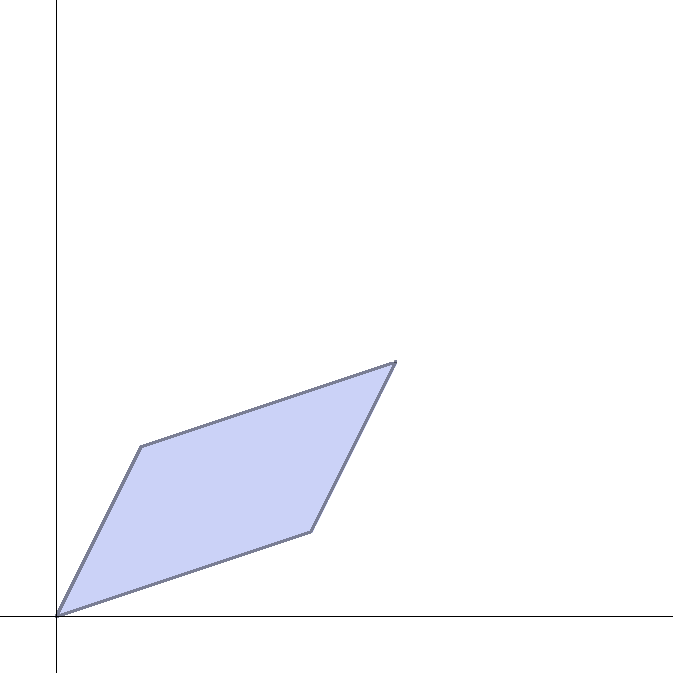
\includegraphics[height = 4truecm, trim = 0 0 80 130, clip]{20150930-fig1.pdf}
\begin{picture}(0,0)
\put(-130, 16.9){\vector(3,1){71.4}}
\put(-130, 16.9){\vector(1,2){23.7}}
\put(-60, 32){$\bm{u}$}
\put(-112, 68){$\bm{v}$}
\end{picture}
\hfil
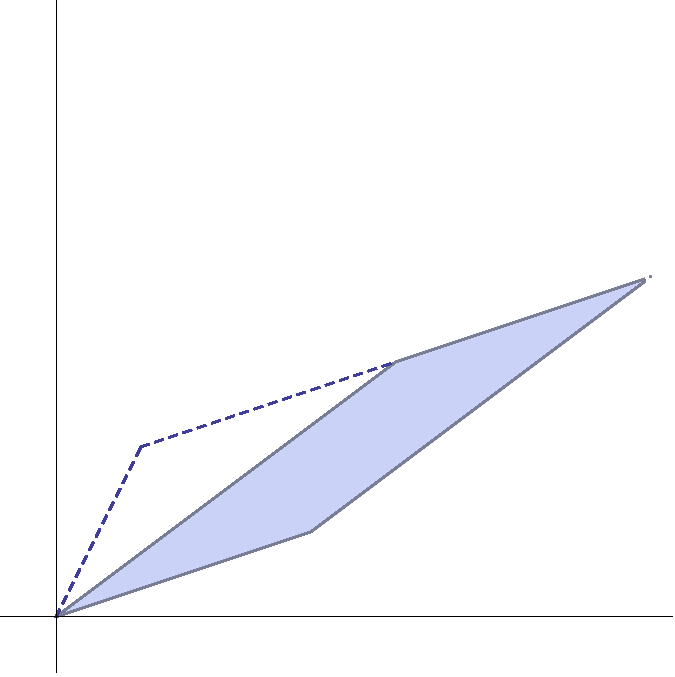
\includegraphics[height = 4truecm, trim = 0 0 0 130, clip]{20150930-fig2.pdf}
\begin{picture}(0,0)
\put(-176.9, 16.8){\vector(3,1){71.4}}
\put(-176.9, 16.8){\vector(4,3){95.1}}
\put(-110, 30){$\bm{u}$}
\put(-95, 95){$\bm{v} + \bm{u}$}
\put(-230, 65){\vector(1, 0){30}}
\end{picture}
\end{figure}

絵で見れば、両方の面積が同じことは明らかですよね。平行四辺形の$1$つの辺を固定して、高さが変形しないように変形しているわけですから。$\alpha$が入った$\det(\bm{u} \ \bm{v} + \alpha \bm{u})$式でも状況は同じです。$\alpha$の値によって平行四辺形がどれだけひしゃげるかが変わるものの、底辺と高さが変わらないようことに変わりはありません。

\paragraph{交代性・多重線型性の面積的意味}

続いて、多重線型性を見てみましょう。まず$\det(\alpha \bm{u} \ \bm{v}) = \alpha \det(\bm{u} \ \bm{v})$という性質がありました。これは$\alpha \bm{u}, \bm{v}$の張る平行四辺形が$\bm{u}, \bm{v}$の張る平行四辺形の$\alpha$倍の面積を持つという意味です。図にしてみれば、明らかでしょう。

\begin{figure}[h!tbp]
\centering
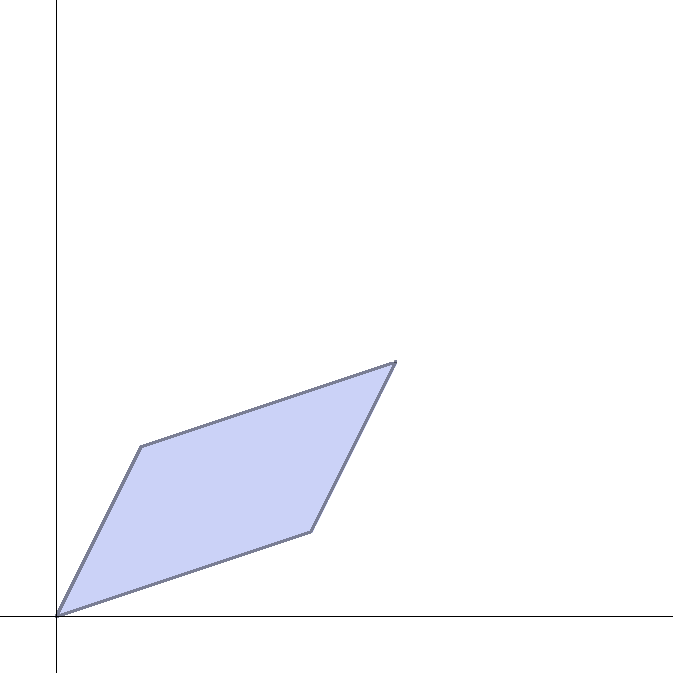
\includegraphics[height = 4truecm, trim = 0 0 80 130, clip]{20150930-fig1.pdf}
\begin{picture}(0,0)
\put(-130, 16.9){\vector(3,1){71.4}}
\put(-130, 16.9){\vector(1,2){23.7}}
\put(-60, 32){$\bm{u}$}
\put(-112, 68){$\bm{v}$}
\end{picture}
\hfil
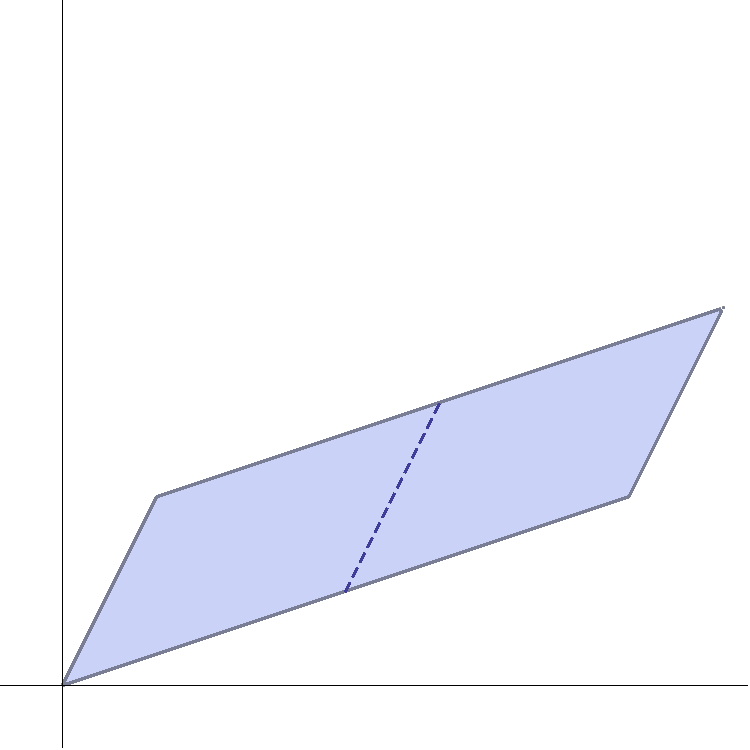
\includegraphics[height = 4truecm, trim = 0 0 0 130, clip]{20150930-fig3.pdf}
\begin{picture}(0,0)
\put(-166.9, 15.2){\vector(3,1){135.2}}
\put(-166.7, 15.2){\vector(1,2){22.5}}
\put(-30, 50){$2\bm{u}$}
\put(-150, 65){$\bm{v}$}
\put(-230, 65){\vector(1, 0){30}}
\end{picture}
\end{figure}

次に、$\det(\bm{u}_1 + \bm{u}_2 \ \bm{v}) = \det(\bm{u}_1 \ \bm{v}) + \det(\bm{u}_2 \  \bm{v})$という式を見てみましょう。
\begin{itemize}
\item $\bm{u}_1$と$\bm{v}$が張る平行四辺形を$S_1$
\item $\bm{u}_2$と$\bm{v}$が張る平行四辺形を$S_2$
\item $\bm{u}_1 + \bm{u}_2$と$\bm{v}$が張る平行四辺形を$S$
\end{itemize}
とおきます。そして$\bm{v}$と垂直な方向の単位ベクトル$\bm{e}$を取っておきます。このとき$\bm{v}$から測った$S_1, S_2$の高さをそれぞれ$l_1$, $l_2$とおくと、$l_1 = |\bm{u}_1 \cdot \bm{e}|$, $l_2 = |\bm{u}_2 \cdot \bm{e}|$です。そして次の図で、$S$の高さ$l_1 - l_2$は$(\bm{u}_1 + \bm{u}_2) \cdot \bm{e}$です。

\begin{figure}[h!tbp]
\centering
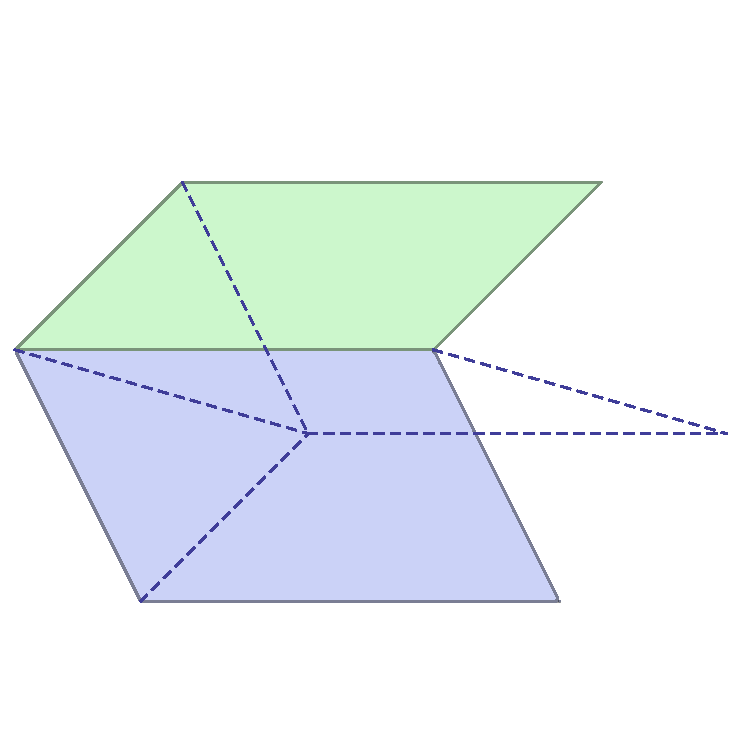
\includegraphics[width = 6truecm, trim = 0 60 0 70, clip]{20150930-fig4.pdf}
\begin{picture}(0,0)
\put(-170.7, 62.7){\vector(1, 0){95.5}}
\put(-170.7, 62.7){\vector(1, 1){38}}
\put(-170.7, 62.7){\vector(1, -2){28.7}}
\put(-190.7, 62.7){\dashbox(20, 0){}}
\put(-170.7, 62.7){\vector(0, -1){20}}
\put(-190.7, 100.7){\dashbox(58, 0){}}
\put(-190.7, 5.3){\dashbox(48.7, 0){}}
\put(-187, 88.7){\vector(0, 1){12}}
\put(-187, 74.7){\vector(0, -1){12}}
\put(-187, 40.3){\vector(0, 1){22.4}}
\put(-187, 27.7){\vector(0, -1){22.4}}
\put(-150, -1){$\bm{u}_1$}
\put(-140, 105){$\bm{u}_2$}
\put(-80, 67){$\bm{v}$}
\put(-189, 78){$l_2$}
\put(-189, 31){$l_1$}
\put(-173,35){$\bm{e}$}
\end{picture}
\hfil
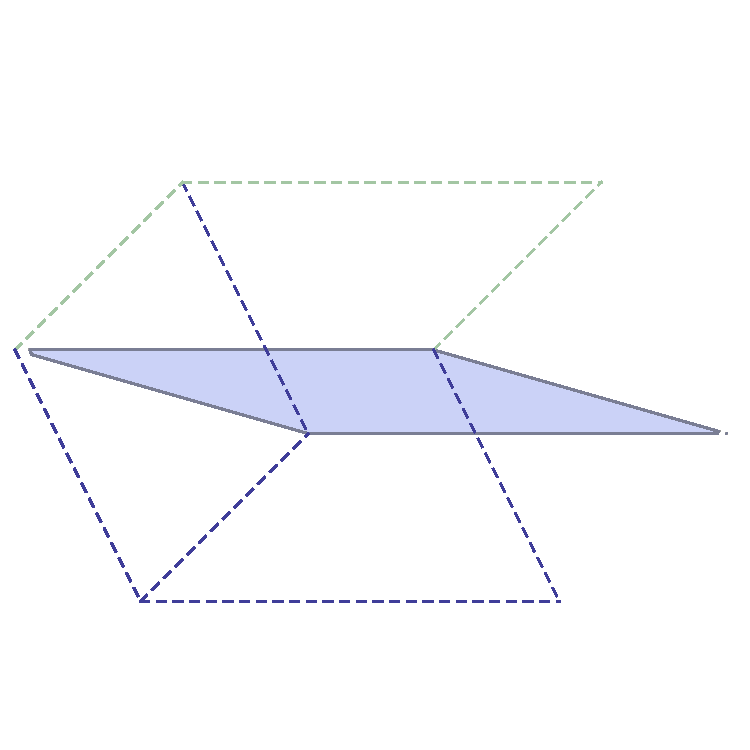
\includegraphics[width = 6truecm, trim = 0 60 0 70, clip]{20150930-fig5.pdf}
\begin{picture}(0,0)
\put(-170.7, 62.7){\vector(1, 0){95.5}}
\put(-170.7, 62.7){\vector(7, -2){66}}
\put(-125, 35){$\bm{u}_1 + \bm{u}_2$}
\put(-80, 67){$\bm{v}$}
\put(-190.7, 62.7){\dashbox(20, 0){}}
\put(-190.7, 43.8){\dashbox(86, 0){}}
\put(-187, 74.7){\vector(0, -1){12}}
\put(-187, 31.8){\vector(0, 1){12}}
\put(-200, 50){$l_1 - l_2$}
\end{picture}
\end{figure}

一般の場合でも同じです。$(\bm{u}_1 + \bm{u}_2) \cdot \bm{e} = \bm{u}_1 \cdot \bm{e} + \bm{u}_2 \cdot \bm{e}$なので、向きまで込めて考えれば$S_1$, $S_2$の高さを足したものが$S$の高さになります。これで$S$の面積が、$S_1$, $S_2$の面積の和であることが示せました。$\det$の言葉で言い換えると、$\det(\bm{u}_1 + \bm{u}_2 \ \bm{v}) = \det(\bm{u}_1 \ \bm{v}) + \det(\bm{u}_2 \  \bm{v})$に他なりません。また$\bm{u}, \bm{v}$を入れ替えると、$\bm{u}$から$\bm{v}$へと回る向きが反転します。この事実を反映して$\det(\bm{u} \ \bm{v}) = - \det(\bm{v} \ \bm{u})$という式が成り立ちます。

\paragraph{体積の持つ交代性・多重線型性}

今の話を、$3$次元でも考えてみましょう。$3$本のベクトル$\bm{u}, \bm{v}, \bm{w}$を引数に取る函数$\vol\colon \mathbb{R}^3 \times \mathbb{R}^3 \times \mathbb{R}^3 \rightarrow \mathbb{R}$を次で定めます。
\begin{itemize}
\item 絶対値は、$\bm{u}, \bm{v}, \bm{w}$の張る平行$6$面体の体積
\item 符号は、$(\bm{u}, \bm{v}, \bm{w})$が右手系のとき$+1$、左手系のとき$-1$
\end{itemize}
\begin{figure}[h!tbp]
\centering
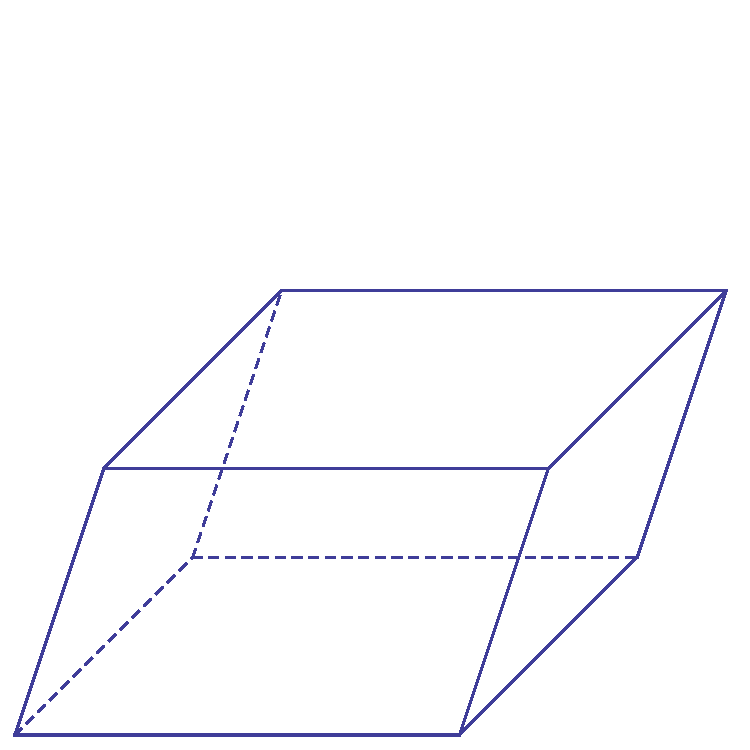
\includegraphics[width = 5truecm, trim = 0 0 0 120, clip]{20150930-fig6.pdf}
\begin{picture}(0, 0)
\put(-142.9, 2.9){\vector(1, 0){84.5}}
\put(-142.7, 2.9){\vector(1, 1){33.7}}
\put(-142.7, 2.9){\vector(1, 3){16.8}}
\put(-66, 7){$\bm{u}$}
\put(-115, 38){$\bm{v}$}
\put(-137, 53){$\bm{w}$}
\end{picture}
\end{figure}

この体積は、作り方から交代性を満たします。右手系をなすベクトルのうち$2$本を入れ替えると、左手系になり、またその逆も成り立つからです。また、$\vol(\bm{u}, \bm{v}, \bm{w})$は$\bm{u}$について線型です。実際$\bm{v}, \bm{w}$の両方に垂直な単位ベクトル$\bm{e}$を取り、$\bm{v}$, $\bm{w}$の張る平行四辺形の面積を$A$とすれば、$\vol(\bm{u}, \bm{v}, \bm{w}) = (\bm{u} \cdot \bm{e}) A$です。この式は$\bm{u}$について線型です。そして交代性から$\vol(\bm{u}, \bm{v}, \bm{w}) = - \vol(\bm{v}, \bm{u}, \bm{w}) = -\vol(\bm{w}, \bm{v}, \bm{u})$だから、$\bm{v}$や$\bm{w}$に対する線型性も従います。

これで$\vol(\bm{u}, \bm{v}, \bm{w})$が交代性と多重線型性の両方を満たすことが言えました。このような性質を持つ函数は$\vol(\bm{u}, \bm{v}, \bm{w}) = \det(\bm{u}\ \bm{v}\ \bm{w}) \vol(\bm{e}_1, \bm{e}_2, \bm{e}_3)$と書けるのでした。そして$\bm{e}_1, \bm{e}_2, \bm{e}_3$の張る平行$6$面体の体積は$1$ですから、$\vol(\bm{u}, \bm{v}, \bm{w}) = \det(\bm{u}\ \bm{v}\ \bm{w})$です。より一般に、$n$次元であっても$\vol = \det$という式が正しいことを示せます。\textbf{体積は交代性と多重線型性を満たすべき}という考察だけから、$\vol = \det$が導かれるのです。

\subsection{$3$次元ベクトルの外積}

$3$次元空間$\mathbb{R}^3$の中の$3$本のベクトル$\bm{a} = {}^t(a_1, a_2, a_3), \bm{b} = {}^t(b_1, b_2, b_3), \bm{c} = {}^t(c_1, c_2, c_3)$を並べた行列の行列式は、$3$列目に関する余因子展開をすることで
\begin{align*}
\det
\begin{pmatrix}
\bm{a} & \bm{b} & \bm{c} 
\end{pmatrix}
&=
\det
\begin{pmatrix}
a_1 & b_1 & c_1 \\
a_2 & b_2 & c_2 \\
a_3 & b_3 & c_3
\end{pmatrix}
= 
c_1 \det
\begin{pmatrix}
a_2 & b_2 \\
a_3 & b_3
\end{pmatrix}
- c_2 \det
\begin{pmatrix}
a_1 & b_1 \\
a_3 & b_3
\end{pmatrix}
+ c_3 \det
\begin{pmatrix}
a_1 & b_1 \\
a_2 & b_2 \\
\end{pmatrix}
\\
&=
c_1 \det
\begin{pmatrix}
a_2 & b_2 \\
a_3 & b_3
\end{pmatrix}
+ c_2 \det
\begin{pmatrix}
a_3 & b_3 \\
a_1 & b_1
\end{pmatrix}
+ c_3 \det
\begin{pmatrix}
a_1 & b_1 \\
a_2 & b_2 \\
\end{pmatrix}
\end{align*}
となります。そこでベクトル$\bm{a} \times \bm{b}$を
\[
\bm{a} \times \bm{b}
:= 
{}^t\biggl(
\det
\begin{pmatrix}
a_2 & b_2 \\
a_3 & b_3
\end{pmatrix}, 
\det
\begin{pmatrix}
a_3 & b_3 \\
a_1 & b_1
\end{pmatrix}, 
\det
\begin{pmatrix}
a_1 & b_1 \\
a_2 & b_2 \\
\end{pmatrix}
\biggr)
\]
と定めると、$(\bm{a} \times \bm{b}) \cdot \bm{c} = \det(\bm{a} \ \bm{b} \ \bm{c})$が成り立ちます\footnote{$(\bm{a} \times \bm{b}) \cdot \bm{c} = \det(\bm{a} \ \bm{b} \ \bm{c})$という式は、よく\textbf{スカラー三重積の公式}と呼ばれます。たとえば電磁気学やベクトル解析の授業などでは、必ず登場すると思います。外積を成分で定義すると$(\bm{a} \times \bm{b}) \cdot \bm{c} = \det(\bm{a} \ \bm{b} \ \bm{c})$が証明できるので「公式」という名前がついています。}。このベクトル$\bm{a} \times \bm{b}$のことを、$\bm{a}$と$\bm{b}$の\textbf{外積}といいます。行列式の交代性を使うと$\det(\bm{a} \ \bm{b} \ \bm{c}) = - \det(\bm{b} \ \bm{a} \ \bm{c})$となるので、$\bm{a} \times \bm{b} = - \bm{b} \times \bm{a}$が分かります。外積は順番をひっくり返せないので、注意してください。

\paragraph{外積の特徴づけ}

$\mathbb{R}^3$のベクトルは向きと大きさで決定されます。そこで外積の向きと大きさを調べてみましょう。

過去に「$\bm{a}$と$\bm{b}$の両方に垂直なベクトル」を作る方法として一度$\bm{a} \times \bm{b}$を紹介したことがありますが、むしろ外積の定義で本質的なのはスカラー三重積の公式$(\bm{a} \times \bm{b}) \cdot \bm{c} = \det(\bm{a} \ \bm{b} \ \bm{c})$です。行列式の交代性を使うと、$\bm{c} = \bm{a}$, $\bm{c} = \bm{b}$とおいたとき、ただちに
\[
(\bm{a} \times \bm{b}) \cdot \bm{a} = \det(\bm{a} \ \bm{b} \ \bm{a}) = 0, 
(\bm{a} \times \bm{b}) \cdot \bm{b} = \det(\bm{a} \ \bm{b} \ \bm{b}) = 0
\]
が分かります。これが$\bm{a} \times \bm{b}$の計算で、$\bm{a}$と$\bm{b}$の両方と垂直なベクトルを作れる理由です。

次に大きさ$|\bm{a} \times \bm{b}|$を考えてみます。$\bm{a}$と$\bm{b}$が平行なら$\bm{a} \times \bm{b} = \bm{0}$なので、そうではないと仮定します。$\bm{a}, \bm{b}, \bm{c}$が$1$次独立になるような$\bm{c} \in \mathbb{R}^3$を取ります。$|\det(\bm{a} \ \bm{b} \ \bm{c})| = |(\bm{a} \times \bm{b}) \cdot \bm{c}|$は$\bm{a}, \bm{b}, \bm{c}$の張る平行$6$面体の体積でした。かたや$\bm{a}, \bm{b}$の張る面の面積を$S$、その面の法線方向と$\bm{c}$のなす角を$[0, \pi/2]$の範囲で測ったものを$\varphi$とすると、平行$6$面体の体積は$S |\bm{c} \cdot \bm{e}| = S|\bm{c}| \cos\varphi$とも表せます。これより
\[
S|\bm{c}| \cos\varphi = |\bm{a} \times \bm{b} \cdot \bm{c}| = |\bm{a} \times \bm{b}| |\bm{c}| \cos \varphi
\]
です。そして$\bm{c}$は$\bm{e}$と垂直にならないよう取っておいたので、$\cos \varphi \neq 0$です。$|\bm{c}| \neq 0$と合わせることで$|\bm{a} \times \bm{b}| = S$が従います。つまり外積は、$\bm{a}, \bm{b}$が張る平行四辺形の面積に一致します。$\bm{a}$と$\bm{b}$のなす角を$\theta$とすれば、$|\bm{a} \times \bm{b}| = |\bm{a}||\bm{b}|\sin\theta$です\footnote{$\bm{a} \cdot \bm{b} = |a||b|\cos\theta$と$\sin \theta = \sqrt{1 - \cos^2\theta}$を使ってゴリゴリ計算しても$|\bm{a} \times \bm{b}|$は求まります。ですが「体積は行列式である」という事実とスカラー三重積の公式を組み合わせれば、大した計算をせずとも綺麗に答えが求まるので、こちらの方法で説明してみました。}。

\begin{figure}[h!tbp]
\centering
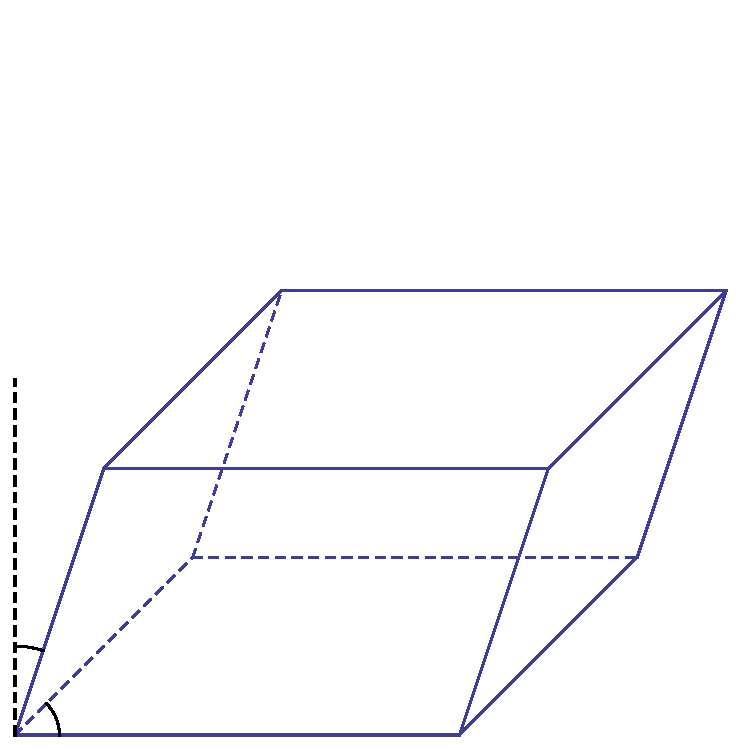
\includegraphics[width = 5truecm, trim = 0 0 0 120, clip]{20150930-fig7.pdf}
\begin{picture}(0, 0)
\put(-142.9, 2.9){\vector(1, 0){84.5}}
\put(-142.7, 2.9){\vector(1, 1){33.7}}
\put(-142.7, 2.9){\vector(1, 3){16.8}}
\put(-66, 7){$\bm{a}$}
\put(-115, 38){$\bm{b}$}
\put(-137, 53){$\bm{c}$}
\put(-142.8, 2.9){\vector(0, 1){40}}
\put(-151, 38){$\bm{e}$}
\put(-141.5, 28){$\varphi$}
\put(-132, 6){$\theta$}
\end{picture}
\end{figure}

最後に行列式の多重線型性を使うと、任意の$\bm{c} \in \mathbb{R}^3$に対し
\begin{align*}
\det\bigl(\bm{a} + \bm{a}'  \ \bm{b} \ \bm{c}\bigr) &= \det(\bm{a} \ \bm{b} \ \bm{c}) + \det(\bm{a}' \ \bm{b} \ \bm{c}) \\
\det(\alpha \bm{a} \ \bm{b} \ \bm{c}) &= \alpha \det(\bm{a} \ \bm{b} \ \bm{c})
\end{align*}
となるから、$\bigl((\bm{a} + \bm{a}') \times \bm{b}\bigr) \cdot \bm{c} = \bigl(\bm{a} \times \bm{b} + \bm{a}' \times \bm{b}\bigr) \cdot \bm{c}$および$\bigl((\alpha \bm{a}) \times \bm{b}\bigr) \cdot \bm{c} = \bigl(\alpha (\bm{a} \times \bm{b})\bigr) \cdot \bm{c}$が成り立ちます。特に$\bm{c}$として標準基底をなす$\bm{e}_1, \bm{e}_2, \bm{e}_3$を取れば、$(\bm{a} + \bm{a}') \times \bm{b}$と$\bm{a} \times \bm{b} + \bm{a}' \times \bm{b}$、$(\alpha \bm{a}) \times \bm{b}$と$\alpha(\bm{a} \times \bm{b})$のそれぞれについて、$x, y, z$成分が一致することが確認できます。これより$(\bm{a} + \bm{a}') \times \bm{b} = \bm{a} \times \bm{b} + \bm{a}' \times \bm{b}$と$(\alpha \bm{a}) \times \bm{b} = \alpha \bm{a} \times \bm{b}$が従います。また
\[
\det (\bm{a} \ \bm{b} \ \bm{a} \times \bm{b}) = (\bm{a} \times \bm{b})\cdot (\bm{a} \times \bm{b}) = |\bm{a} \times \bm{b}|^2 = |\bm{a}|^2 |\bm{b}|^2 \sin^2 \theta
\]
です。$\bm{a}, \bm{b}$が$1$次独立なら$|\bm{a}|, |\bm{b}| \neq 0$かつ$\theta \neq 0, \pi$なので$\bm{a} \times \bm{b} \neq \bm{0}$です。よって$\bm{a}, \bm{b}$が$1$次独立なとき、$\bm{a}, \bm{b}, \bm{a} \times \bm{b}$をこの順に並べると右手系\footnote{この部分では「$\det > 0$だから右手系」という書き方をしていますが、実は逆です。$1$次独立な$3$本のベクトル$\bm{a}, \bm{b}, \bm{c}$が右手系であることを、$\det(\bm{a} \ \bm{b} \ \bm{c}) > 0$で定義します。こうすると「右手の法則にしたがう」という曖昧な言い方を回避してきちんと定義ができ、さらに「右手系と左手系がきちんと区別されること」「右手系と左手系以外の○○系がないこと」などが示せます。将来「内積」の話をする際、一緒に「空間の向き」のことを紹介します。}をなします。これで$\bm{a} \times \bm{b}$の向きが完全に決定されました。

かくして外積$\bm{a}, \bm{b}$は
\begin{itemize}
\item 大きさが$\bm{a}, \bm{b}$の張る平行四辺形の面積
\item $\bm{a}, \bm{b}$の両方と垂直な向き
\item $\bm{a}, \bm{b}, \bm{a} \times \bm{b}$が右手系
\end{itemize}
という条件で特徴づけられるベクトルだということも分かりました。

\section{おまけ: A2ターム期末試験の解説}

「A2タームの期末試験の解説がほしい」というリクエストをいただいたので、解答と解説を作りました。復習に役立ててください。なお配点がどうなっているのかはそもそも知らないので、書いていません。

\subsection{問1}

(2) は中々難しいと思います。$|z| = 1$となる複素数は$\cos\theta + i \sin\theta$と表せますが、$\theta$をパラメータに取った状態では$\cos \theta$と$\sin \theta$の両方を同時が有理数になるタイミングは見えてきません。ここで三角函数の入った積分を置換積分で解くときに、たまに使う公式を思い出します。$t := \tan (\theta/2)$とおくと
\[
\cos \theta = \frac{1 - t^2}{1 + t^2}, \quad \sin \theta = \frac{2t}{1 + t^2}
\]
が成り立つのを、覚えていますか?この式は大変都合の良いことに、$t$の有理式です。したがって$t$が有理数であれば、$\cos \theta$と$\sin \theta$が両方とも有理式になることが分かります。そうすれば後は、$t$が有理数になるような$\theta$が無限個存在することを示すだけです。

\paragraph{解答}
\noindent (1) $(a + bi)\overline{(a + bi)} = a^2 + b^2$を使うと (a) 2, (b) 5, (c) 13 と分かる。

\noindent (2) $(1 - t^2)^2 + (2t)^2 = (1 + t^2)^2$の両辺を$1 + t^2$で割ると
\[
\biggl(\frac{1 - t^2}{1 + t^2}\biggr)^2 + \biggl(\frac{2t}{1 + t^2}\biggr)^2 = 1
\]
となる。よって実数$t$に対し
\[
z(t) := \frac{1 - t^2}{1 + t^2} + \frac{2t}{1 + t^2}i
\]
と定めると、$t$の値が何であっても$|z(t)| = 1$である。式の形から、$t$が有理数なら$z(t)$の実部、虚部は共に有理数である。そして
\[
\mathrm{Re}\, z(t) = \frac{2}{1 + t^2} - 1
\]
は$t$について単調減少で、$\mathrm{Re}\, z(0) = 1$, $\mathrm{Re}\, z(1) = 0$である。したがって閉区間$[0, 1]$の点$t$に$z(t)$を対応させる写像は単射である。これと$[0, 1]$に有理数が無数に存在することから、求める結果を得る。\qed

\subsection{問2}

この問題については、特に注釈は要らないでしょう。地道に計算するだけです。

\paragraph{解答}

\noindent (1) 
$\overrightarrow{\mathrm{\,AB\,}} = {}^t(\sqrt{2} - 1 ,\sqrt{3} - \sqrt{2} ,1 - \sqrt{3})$, $\overrightarrow{\mathrm{\,AC\,\,}} = {}^t(\sqrt{3} - 1, 1 - \sqrt{2}, \sqrt{2} - \sqrt{3})$なので
\begin{align*}
\cos\angle\mathrm{BAC} = \frac{\overrightarrow{\mathrm{\,AB\,}}\cdot \overrightarrow{\mathrm{\,AC\,\,}}}{\bigl|\overrightarrow{\mathrm{\,AB\,}}\bigr|\bigl|\overrightarrow{\mathrm{\,AC\,\,}}\bigr|}
&= \frac{(\sqrt{2} - 1)(\sqrt{3} - 1) + (\sqrt{3} - \sqrt{2})(1 - \sqrt{2}) + (1 - \sqrt{3})(\sqrt{2} - \sqrt{3})}{(\sqrt{2} - 1)^2 + (\sqrt{3} - \sqrt{2})^2 + (1 - \sqrt{3})^2} \\
&= \frac{(\sqrt{2} - 1)^2 + (1 - \sqrt{3})(\sqrt{2} - \sqrt{3})}{12 - 2(\sqrt{2} + \sqrt{3} + \sqrt{6})}
= \frac{6 - \sqrt{2} - \sqrt{3} - \sqrt{6}}{12 - 2(\sqrt{2} + \sqrt{3} + \sqrt{6})} \\
&= \frac{1}{2}
\end{align*}
となる。よって$\angle\mathrm{BAC} = \pi/3$である。

\noindent (2) $\alpha \bm{a} + \beta (\bm{a} + \bm{b}) = \bm{0}$とおく。このとき$(\alpha + \beta)\bm{a} + \beta \bm{b} = \bm{0}$なので、$\bm{a}, \bm{b}$の$1$次独立性から$\alpha + \beta = 0, \beta = 0$が従う。これを解くと$\alpha = \beta = 0$となる。よって$\bm{a}, \bm{a} + \bm{b}$は$1$次独立である。

\noindent (3) $2\bm{a} + t(\bm{b} - 2\bm{a}) = \bm{a} + s(\bm{a} + 3\bm{b})$のとき、$(1 - 2t - s)\bm{a} + (t - 3s)\bm{b} = \bm{0}$となる。よって$\bm{a}, \bm{b}$の$1$次独立性から$2t + s = 1$, $t - 3s = 0$という連立方程式を得る。これを解いて$s = 1/7, t = 3/7$を得る。 \qed

\subsection{問3} ただの計算問題です。下三角同士の積が再び下三角行列になることを覚えていると、(2) では対角線より上の計算を端折れます。

\paragraph{解答}

\begin{align*}
\frac{1}{2}
\begin{pmatrix}
1 & 4 & 7 \\
2 & 5 & 8 \\
3 & 6 & 9
\end{pmatrix}
- \frac{1}{2}
\begin{pmatrix}
1 & 2 & 3 \\
4 & 5 & 6 \\
7 & 8 & 9
\end{pmatrix}
&=
\begin{pmatrix}
0 & 1 & 2 \\
-1 & 0 & 1 \\
-2 & -1 & 0
\end{pmatrix} \\
\begin{pmatrix}
1 & 0 & 0 \\
1 & 1 & 0 \\
1 & 2 & 1
\end{pmatrix}
\begin{pmatrix}
1 & 0 & 0 \\
-1 & 1 & 0 \\
1 & -2 & 1
\end{pmatrix}
&=
\begin{pmatrix}
1 & 0 & 0 \\
0 & 1 & 0 \\
-1 & 2 & 1
\end{pmatrix} \\
\begin{pmatrix}
\sqrt{2} & -1 & 1 \\
\sqrt{2} & 1 & -1 \\
0 & \sqrt{2} & \sqrt{2}
\end{pmatrix}
\begin{pmatrix}
\sqrt{2} & \sqrt{2} & 0 \\
-1 & 1 & \sqrt{2} \\
1 & -1 & \sqrt{2}
\end{pmatrix}
&= 
\begin{pmatrix}
4 & 0 & 0 \\
0 & 4 & 0 \\
0 & 0 & 4
\end{pmatrix}
\end{align*}
\qed

\subsection{問4}

拡大係数行列に未知数$a$が入り込んでいるのがややこしいところです。$a$の値によって、係数行列や拡大係数行列の$\rank$が変わることが予想されます。

なるべく手間をかけたくないので、式中に$a$を残したまま、できる限り行基本変形を進めてみましょう。その際\textbf{$a$の入った式で割り算をしないこと}が大事です。たとえば$a - 1$が$0$だろうがそれ以外だろうが、「ある行の$a - 1$倍を別の行に足す」という操作はできます。しかし$a - 1 = 0$のときは「$a - 1$で割る」という操作をすると破綻が生じてしまいます。

\paragraph{解答} まず、拡大係数行列を次のように行基本変形する
\begin{align*}
\left(\begin{array}{cccc|c}
1 & 1 & 1 & 1 & 1 \\
a & 1 & 1 & 1 & 1 \\
1 & a & 3 - a & 1 & 3 \\
2 & 2 & a & 2 & 0
\end{array}\right)
\xrightarrow[\text{\hbox to 10zw{\hfil $1$列目を掃き出す \hfil}}]{\text{\hbox to 10zw{\hfil $(1, 1)$成分を要に \hfil}}} & 
\left(\begin{array}{cccc|c}
1 & 1 & 1 & 1 & 1 \\
0 & 1 - a & 1 - a & 1 - a & 1 - a \\
0 & a - 1 & 2 - a & 0 & 2 \\
0 & 0 & a - 2 & 0 & -2
\end{array}\right) \\
\xrightarrow[\text{\hbox to 10zw{\hfil 加える \hfil}}]{\text{$2$行目を$3$行目に}} & 
\left(\begin{array}{cccc|c}
1 & 1 & 1 & 1 & 1 \\
0 & 1 - a & 1 - a & 1 - a & 1 - a \\
0 & 0 & 3 - 2a & 1 - a & 3 - a \\
0 & 0 & a - 2 & 0 & -2
\end{array}\right) \\
\xrightarrow[\text{\hbox to 10zw{\hfil $2$倍を加える \hfil}}]{\text{$3$行目に$4$行目の}} & 
\left(\begin{array}{cccc|c}
1 & 1 & 1 & 1 & 1 \\
0 & 1 - a & 1 - a & 1 - a & 1 - a \\
0 & 0 & -1 & 1 - a & -1 - a \\
0 & 0 & a - 2 & 0 & -2
\end{array}\right) \\
\xrightarrow[\text{\hbox to 10zw{\hfil $a - 2$倍を加える \hfil}}]{\text{$4$行目に$3$行目の}} & 
\left(\begin{array}{cccc|c}
1 & 1 & 1 & 1 & 1 \\
0 & 1 - a & 1 - a & 1 - a & 1 - a \\
0 & 0 & -1 & 1 - a & - 1 - a \\
0 & 0 & 0 & (1 - a)(a - 2) & -a(a - 1)
\end{array}\right) \\
\end{align*}
この式より、係数行列の$\rank$が$a = 1, 2$とそれ以外で変化しそうだと分かる。
\begin{itemize}
\item $a = 1$のとき、拡大係数行列は
\[
\left(\begin{array}{cccc|c}
1 & 1 & 1 & 1 & 1 \\
0 & 0 & 0 & 0 & 0 \\
0 & 0 & -1 & 0 & - 2 \\
0 & 0 & 0 & 0 & 0
\end{array}\right)
\]
となる。よって係数行列と拡大係数行列の$\rank$は共に$2$である。
\item $a = 2$のとき、拡大係数行列は
\[
\left(\begin{array}{cccc|c}
1 & 1 & 1 & 1 & 1 \\
0 & -1 & -1 & -1 & -1 \\
0 & 0 & -1 & -1 & -3 \\
0 & 0 & 0 & 0 & -1
\end{array}\right)
\]
となる。$(2, 2)$成分と$(3, 3)$成分を要にして$2$列目と$3$列目を掃き出してから、符号を調整すると
\[
\left(\begin{array}{cccc|c}
1 & 0 & 0 & * & * \\
0 & 1 & 0 & * & * \\
0 & 0 & 1 & * & * \\
0 & 0 & 0 & 0 & 1
\end{array}\right)
\]
の形に変形できる。よって係数行列の$\rank$は$3$で、拡大係数行列の$\rank$は$4$である。
\item それ以外の場合$a - 1, a - 2 \neq 0$なので、$2$行目を$1 - a$で、$4$行目を$(1 - a)(a - 2)$で割ってよい。
\[
\left(\begin{array}{cccc|c}
1 & 1 & 1 & 1 & 1 \\
0 & 1 & 1 & 1 & 1 \\
0 & 0 & 1 & a - 1 & 1 + a \\
0 & 0 & 0 & 1 & a/(2 - a)
\end{array}\right)
\]
この後$(1, 1)$成分から$(4, 4)$成分までを順番に要として$1$列目から$4$列目を掃き出せば
\begin{align*}
\left(\begin{array}{cccc|c}
1 & 1 & 1 & 1 & 1 \\
0 & 1 & 1 & 1 & 1 \\
0 & 0 & 1 & a - 1 & 1 + a \\
0 & 0 & 0 & 1 & a/(a - 2)
\end{array}\right)
&\rightarrow
\left(\begin{array}{cccc|c}
1 & 0 & 0 & 0 & 0 \\
0 & 1 & 0 & 2 - a & -a \\
0 & 0 & 1 & a - 1 & 1 + a \\
0 & 0 & 0 & 1 & a/(a - 2)
\end{array}\right)
\rightarrow
\left(\begin{array}{cccc|c}
1 & 0 & 0 & 0 & 0 \\
0 & 1 & 0 & 0 & 0 \\
0 & 0 & 1 & 0 & -2/(a - 2) \\
0 & 0 & 0 & 1 & a/(a - 2)
\end{array}\right)
\end{align*}
となる。よって係数行列の$\rank$は$4$である。拡大係数行列の$\rank$は係数行列の$\rank$以上で、かつ行数以下である。よって拡大係数行列の$\rank$もまた$4$になる。
\end{itemize}

\noindent (2), (3) 行列が解を持つための必要十分条件は、係数行列と拡大係数行列の$\rank$が一致することであった。したがって解が存在するための条件は$a \neq 2$である。また解がただ$1$つ存在するための必要十分条件は、係数行列が正方行列で、かつ係数行列の$\rank$が行列のサイズと一致することである。よって$a \neq 1, 2$のとき、解はただ$1$つに定まる。

$a \neq 1, 2$のとき、解は上で計算した通り
\[
x = y = 0, z = -\frac{2}{a - 2}, w = \frac{a}{a - 2}
\]
である。また$a = 1$のときは、行基本変形後の拡大係数行列を見れば、$x, y$は任意で
\[
z = 2, w = - 1 - x - y
\]
が解だと分かる。\qed

\subsection{問5}
\noindent (1)
\[
\begin{pmatrix}
\bm{u}_1 & \bm{u}_2 & \bm{u}_3
\end{pmatrix}
=
\begin{pmatrix}
1 & 0 & 1 \\
2 & 1 & 0 \\
0 & 1 & -1
\end{pmatrix}
\]
の逆行列を求めるには、右側に単位行列を並べて、左側の行列が単位行列になるよう行基本変形を行えば良い。
\begin{align*}
\left(
\begin{array}{rrr|rrr}
1 & 0 & 1 & 1 & 0 & 0 \\
2 & 1 & 0 & 0 & 1 & 0 \\
0 & 1 & -1 & 0 & 0 & 1
\end{array}
\right)
&\rightarrow
\left(
\begin{array}{rrr|rrr}
1 & 0 & 1 & 1 & 0 & 0 \\
0 & 1 & -2 & -2 & 1 & 0 \\
0 & 1 & -1 & 0 & 0 & 1
\end{array}
\right) \\
&\rightarrow
\left(
\begin{array}{rrr|rrr}
1 & 0 & 1 & 1 & 0 & 0 \\
0 & 1 & -2 & -2 & 1 & 2 \\
0 & 0 & 1 & 2 & -1 & 1
\end{array}
\right)
\rightarrow
\left(
\begin{array}{rrr|rrr}
1 & 0 & 0 & -1 & 1 & -1 \\
0 & 1 & 0 & 2 & -1 & 2 \\
0 & 0 & 1 & 2 & -1 & 1
\end{array} \right)
\end{align*}

\noindent (2) $T$の表現行列を$A$と書くと
\[
A =
\begin{pmatrix}
1 & 1 & 1 \\
1 & 2 & 0 \\
0 & 1 & -1
\end{pmatrix}
\]
である。

\noindent (3) $A$を行基本変形すると
\[
\begin{pmatrix}
1 & 1 & 1 \\
1 & 2 & 0 \\
0 & 1 & -1
\end{pmatrix}
\rightarrow
\begin{pmatrix}
1 & 1 & 1 \\
0 & 1 & -1 \\
0 & 1 & -1
\end{pmatrix}
\rightarrow
\begin{pmatrix}
1 & 0 & 2 \\
0 & 1 & -1 \\
0 & 0 & 0
\end{pmatrix}
\]
となる。よって$A\bm{x} = 0$の解は
\[
\bm{x} = 
\begin{pmatrix}
-2z \\
z \\
z
\end{pmatrix}
=
z
\begin{pmatrix}
-2 \\
1 \\
1
\end{pmatrix}
\]
と書ける。よって基底として$-2 \bm{u}_1 + \bm{u}_2 + \bm{u}_3$が取れる。

\noindent (4) $\dim \Im T = 3 - \dim \Ker T = 2$である。よって$A$の列ベクトルのうち一次独立な$2$本を取れば、それが基底になる。
\[
\det
\begin{pmatrix}
1 & 1 \\
1 & 2
\end{pmatrix}
= 2 - 1 = 1 \neq 0
\]
より、最初の$2$本が$1$次独立である。よって基底として$\bm{u}_1 + \bm{u}_2$, $\bm{u}_1 + 2\bm{u}_2 + \bm{u}_3$が取れる。


